%-----------------------------------------------------------------------------%
\chapter{ANALISIS DAN PERANCANGAN SISTEM}

%-----------------------------------------------------------------------------%

%
\vspace{4.5pt}

Bab ini menjelaskan analisis masalah beserta pendekatan dan alur kerja dari aplikasi yang akan dikembangkan, dimulai dari \textit{preprocessing}, implementasi metode dan hasil yang ditampilkan.
\section{Analisis Masalah}
Dalam penelitian ini, penulis akan menggunakan data berupa \textit{tweet} dari media sosial Twitter untuk data \textit{training} dan data \textit{testing}. Penulis memilih media sosial Twitter sebagai objek penelitian, karena Twitter memiliki fitur \textit{hashtag} yang dapat digunakan untuk mendapatkan data sarkasme, yang kemunculannya sedikit. Selain itu, pada tahun 2011 tercatat ada 200 juta \textit{tweet} setiap harinya. Penulis akan menggunakan klasifikasi \textit{Support Vector Machine} (SVM) pada pengembangan \textit{sistem} analisis sentimen ini. \textit{Kernel} SVM yang dipilih adalah linear, karena jumlah fitur lebih banyak dibanding jumlah data. Data diambil dengan \textit{scraping} html pada halaman Twitter menggunakan \textit{library} Python, yaitu Twitter-scraper. Data diambil berdasarkan pencarian pada Twitter dengan berbagai \textit{keyword}. \textit{Keyword} yang digunakan adalah "DPR", "film", "sekolah" dan "internet" untuk mendapatkan data dengan label positif, negatif 
dan netral. Sedangkan data dengan label sarkasme diambil dengan menggunakan \textit{keyword} seperti "DPR \#sarkasme", "film \#sarkasme", "sekolah \#sarkasme", dan "internet \#sarkasme". Digunakannya \textit{keyword} tersebut karena \textit{keyword} 
tersebut memiliki cukup banyak data sarkasme, dengan 13 teks sarkasme pada \textit{keyword }DPR, 3 teks sarkasme pada \textit{keyword} film, 12 teks sarkasme pada \textit{keyword} sekolah dan 7 teks sarkasme pada \textit{keyword} internet. Dalam penelitian ini akan dilakukan klasifikasi dengan 2 teknik klasifikasi, yaitu \textit{levelled method} dan \textit{direct method} \cite{5}. Pengklasifikasian akan menganggap teks sarkasme sebagai positif sarkasme, karena teks sarkasme cenderung terlihat seperti teks positif, namun bernilai negatif \cite{5}. Berikut ini adalah \textit{flowchart }
proses klasifikasi dengan \textit{levelled method}:

\begin{adjustbox}{width=1\textwidth}
\begin{minipage}{\linewidth}
	\framebox[\textwidth]{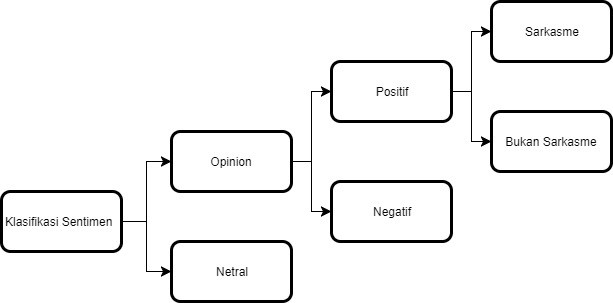
\includegraphics[width=10cm]{images/levelled_method.jpg}}	
	\captionof{figure}{Klasifikasi dengan \textit{Levelled Method}}
\end{minipage}
\end{adjustbox}

Berikut ini adalah \textit{flowchart }proses klasifikasi dengan \textit{direct method}:

\begin{adjustbox}{width=1\textwidth}
\begin{minipage}{\linewidth}
	\framebox[\textwidth]{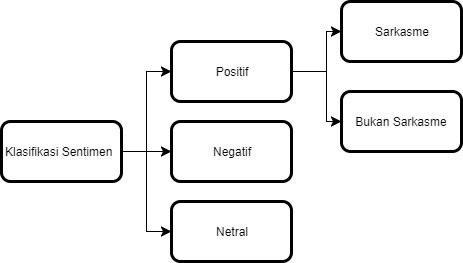
\includegraphics[width=10cm]{images/direct_method.jpg}}	
	\captionof{figure}{Klasifikasi dengan \textit{Levelled Method}}
\end{minipage}
\end{adjustbox}

Klasifikasi \textit{levelled method} dan \textit{direct method }akan membangun sebanyak 4 model. Berikut ini adalah model yang diperlukan untuk klasifikasi \textit{levelled method }dan \textit{direct method}:

\begin{enumerate}[leftmargin=*]
	\item Model 1\ \ \ \ : kelas netral atau bukan netral.
	\item Model 2\ \ \ \ : kelas positif atau bukan positif.
	\item Model 3\ \ \ \ : kelas negatif atau bukan negatif.
	\item Model 4\ \ \ \ : kelas sarkasme atau bukan sarkasme.
\end{enumerate}

Pada klasifikasi \textit{levelled method }akan dilakukan klasifikasi teks termasuk sebagai kelas netral atau kelas opini. Jika teks merupakan kelas opini, maka akan diklasifikasikan menjadi teks positif atau negatif. Jika hasilnya kelas positif, maka akan diklasifikan menjadi teks sarkasme atau non-sarkasme. Sedangkan pada klasifikasi \textit{direct method} teks akan langsung diklasifikasikan sebagai 3 kelas, yaitu positif, negatif atau netral. Jika teks merupakan positif, maka akan diklasifikasikan sebagai sarkasme atau non-sarkasme. Penelitian ini akan membandingkan akurasi klasifikasi \textit{levelled method} dan \textit{direct method}.

Data \textit{tweet} yang dikumpulkan akan diberi label secara manual. Data \textit{tweet} yang diambil tersebut diberi label sebagai positif, negatif, netral, sarkasme. Salah satu fitur yang dianggap membantu dalam penentuan teks sarkasme adalah menggunakan fitur seperti \textit{emoticon}, kemunculan kata \textit{adjective }dan \textit{adverb, }kemunculan \textit{interjection }dan penggunaan \textit{punctuation }\cite{5}. Fitur-fitur yang akan digunakan pada penelitian ini adalah \textit{unigram,} \textit{interjection}, \textit{question word,} \textit{sentiment score, capitalization},
\textit{ topic}, \textit{part of speech} dan \textit{punctuation-based}. Fitur \textit{unigram }lebih dipilih dibanding \textit{bigram},\textit{ }karena kata-kata pada media social terlalu beragam, sehingga sulit untuk menemukan kata yang sama jika 
menggunakan \textit{bigram}. Berikut ini adalah contoh teks yang akan menganggap sebuah kata beda jika menggunakan \textit{bigram}:

\begin{enumerate}[leftmargin=*]
	\item Se7...kalau boleh setiap hari kemerdekaan WAJIB TAYANG \textbf{DI 
		SEKOLAH}
	\item Ceritanya menarik. Karakternya juga unik. Salah satu karakter 
	favorit, Endong. Aktingnya cukup keren. Sangat cocok di tonton \textbf{
		anak sekolah}.
	\item Tiap sore \textbf{pulang} \textbf{sekolah} ngarepin paket 
	dating
\end{enumerate}

Berdasarkan data di atas, jika menggunakan \textit{bigram}, akan menghasilkan token ["tayang sekolah"], ["anak sekolah"], dan ["pulang sekolah"]. Hal tersebut menyebabkan setiap token tersebut akan dianggap berbeda dan nilai fitur tidak bagus. Kata "di" pada teks 1 dihapus, karena kata "di" tidak memiliki makna, oleh karena itu fitur kata \textit{bigram} menjadi ["tayang sekolah"]. Sedangkan jika menggunakan \textit{unigram}, akan menghasilkan token ["tayang", "sekolah"], ["anak", "sekolah"], dan ["pulang", "sekolah"]. Sehingga kata "sekolah" dapat memberikan nilai fitur yang lebih baik karena kemunculannya adalah 3.

\pagebreak

\section{Kerangka Pemikiran}
Berikut ini adalah kerangka pemikiran dari metode yang diusulkan untuk 
melakukan klasifikasi:

\begin{adjustbox}{width=1\textwidth}
\begin{minipage}{\linewidth}
	\framebox[\textwidth]{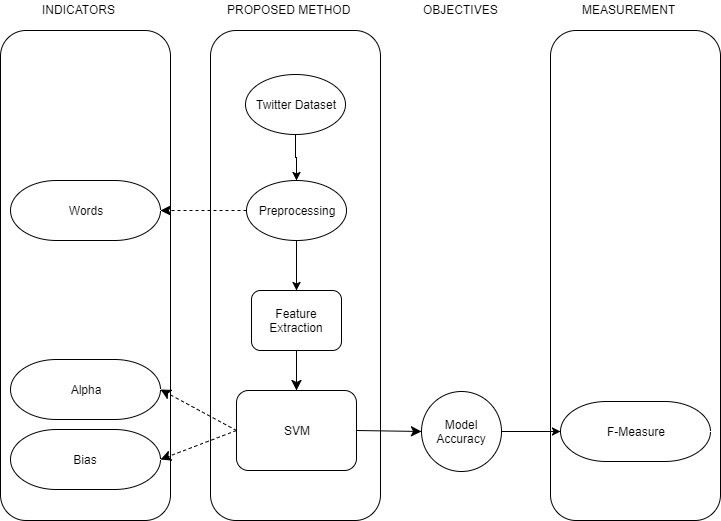
\includegraphics[width=10cm,height=8cm]{images/kerangka_pemikiran.jpg}}	
	\captionof{figure}{Kerangka kerja klasifikasi teks}
\end{minipage}
\end{adjustbox}

Sistem akan dimulai dari masukan data Twitter. Kemudian melakukan proses \textit{text preprocessing} dengan menggunakan data Twitter yang sudah diberi label. Tahap selanjutnya setelah \textit{preprocessing} adalah melakukan \textit{feature extraction}. Hasil \textit{feature extraction }akan digunakan untuk pemodelan klasifikasi SVM. Setelah mendapatkan modelnya, maka dapat dihitung akurasinya dengan \textit{f-measure}.
 
\section{\textit{Flowchart} Sistem Analisis Sentimen}
Berikut adalah flowchart untuk sistem analisis sentimen dalam penelitian 
ini:

\begin{adjustbox}{width=1\textwidth}
\noindent\begin{minipage}{\linewidth}
	\framebox[\textwidth]{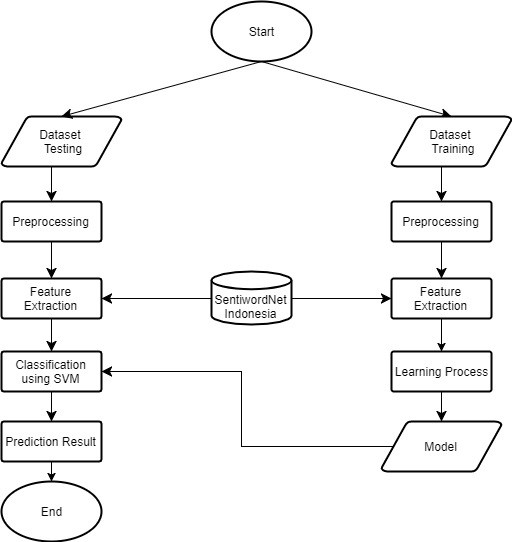
\includegraphics[width=10cm]{images/flowchart.jpg}}	
	\captionof{figure}{\textit{Flowchart} Sistem Analisis Sentimen}
\end{minipage}
\end{adjustbox}

Alur proses sistem dimulai dari data \textit{training}. Kemudian dilanjutkan dengan \textit{preprocessing}. Setelah itu, data \textit{training} yang sudah di \textit{preprocessing }akan masuk ke tahap \textit{feature extraction} untuk mendapatkan informasi dari setiap teks. \textit{Feature extraction }akan menggunakan data SentiWordNet untuk mendapatkan fitur nilai sentimen dari sebuah teks. Kemudian melakukan \textit{learning process} untuk menghasilkan model klasifikasi SVM. Setelah model didapatkan, data \textit{testing} dapat melakukan tahap-tahap seperti pada data \textit{training}, yaitu \textit{preprocessing }dan\textit{ feature extraction}. Setelah mendapat fitur dari data \textit{testing}, selanjutnya dapat melakukan klasifikasi teks dengan model yang sudah melalui \textit{learning process}. 

\subsection{Analisis Data}
Dalam penelitian ini, akan digunakan 236 data \textit{tweet} yang sudah diberi kelas pada setiap \textit{tweet}. Kelas tersebut dibagi menjadi 4 kelas yaitu, kelas positif, kelas negatif, kelas netral dan kelas sarkasme. Selain itu, akan digunakan 177 data \textit{tweet} sebagai data training, dan 59 data \textit{tweet} sebagai data \textit{testing}. Berikut contoh dari data \textit{tweet} yang akan digunakan:

\begin{enumerate}[leftmargin=*]
	\item Kelas Positif\\
	Sukses untuk pak @aniesbaswedan, stop reklamasi !!
	\item Kelas Negatif\\
	Anggota DPR skrg tidak mementingkan rakyat.
	\item Kelas Netral\\
	Menurut Netizen, Apakah DPR RI/DPRD sudah mewakili aspirasi rakyat?
	\item Kelas Sarkasme\\
	Semoga FH dan FZ ada di DPR selamanya.. krn sepi dunia kalau gak ada mereka.. :)
\end{enumerate}

\noindent Karakteristik data yang digunakan:
\begin{enumerate}[leftmargin=*]
	\item Semua sarkasme akan dianggap sebagai sarkasme positif.
	\item Jika ada perbandingan pada sebuah kalimat, pemberian label 
	berdasarkan kalimat yang lebih memberi nilai positif maupun negatif, 
	sebagai contoh \textit{tweet} "Tapi, penilaian sy kinerja 
	pemerintahan dan kpk lebih baik daripada yang di dpr", teks tersebut 
	akan diberi label positif.
\end{enumerate}
		
\subsection{\textit{Text Preprocessing}}
Sebelum melakukan ekstraksi fitur, akan dilakukan \textit{text} \textit{preprocessing }pada data \textit{training} dan data \textit{testing}. \textit{Text preprocessing }dilakukan untuk mengurangi \textit{noise}, dan mengurangi kata-kata non-formal. Beberapa metode untuk menangani \textit{noise} atau kata-kata non-formal pada \textit{text preprocessing }seperti \textit{case folding, remove hashtag}, URL dan \textit{mention}, \textit{remove punctuation}, \textit{tokenization}, \textit{misuse of word}, \textit{abbreviation word}, \textit{stopword removal}, dan \textit{stemming}. Berikut ini adalah \textit{flowchart text preprocessing} yang akan dilakukan:

\begin{adjustbox}{width=1\textwidth}
\begin{minipage}{\linewidth}
	\framebox[\textwidth]{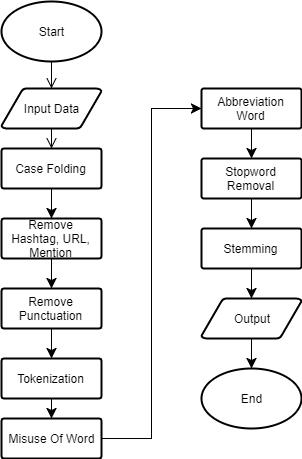
\includegraphics[width=10cm,height=10cm]{images/text_preprocessing.png}}	
	\captionof{figure}{\textit{Flowchart Text Preprocessing}}
\end{minipage}
\end{adjustbox}

\subsubsection{\textit{Case Folding}}
Pada tahap \textit{Case Folding, }kalimat pada teks akan diubah menjadi huruf kecil. \textit{Case folding }dilakukan untuk mengatasi masalah kata yang sama, hanya berbeda huruf kapital.

\begin{table}[H]
	\caption{Tabel Hasil \textit{Case Folding}}
	\centering
	\small
	\begin{adjustbox}{width=1\textwidth}
	\begin{tabular}{|p{6.50cm}|p{6.50cm}|}
		\hline
		\textbf{Teks} & \textbf{Hasil} \\
		\hline
		\textbf{BPK} terbaik. \textbf{BI} terbaik. \textbf{DPR} ter? \textbf{@Fahrihamzah} ter? \textbf{Mandi} dlu \textbf{Ooom!} 
		& \textbf{bpk} terbaik. \textbf{bi} terbaik. \textbf{dpr} ter? \textbf{@fahrihamzah} ter? \textbf{mandi} dlu \textbf{ooom!} \\
		\hline
	\end{tabular}
	\end{adjustbox}
\end{table}
\subsubsection{\textit{Remove Hashtag}, URL, \textit{Mention}}
Pada tahap ini, semua \textit{hashtag}, URL, \textit{mention} akan dihapus dari teks. Penghapusan ini dilakukan karena dalam teks sarkasme sering terdapat \textit{hashtag} \#sarkasme, hal ini dapat membantu dalam sebuah fitur jika tidak menghapusnya. Namun setiap teks yang memiliki \textit{hashtag} \#sarkasme, tidak menentukan bahwa sebuah 
teks adalah sarkasme, sehingga \textit{hashtag} akan dihapus. Berikut ini adalah contoh hasil \textit{remove hashtag}, URL, dan \textit{mention}:
\begin{table}[H]
	\caption{Tabel Hasil \textit{Remove Hashtag}, URL, \textit{Mention}}
	\centering
	\small
	\begin{adjustbox}{width=1\textwidth}
	\begin{tabular}{|p{6.50cm}|p{6.50cm}|}
		\hline
		\textbf{Teks} & \textbf{Hasil} \\
		\hline
		bpk terbaik. bi terbaik. dpr ter? \textbf{@fahrihamzah} ter? mandi dlu ooom! & bpk terbaik. bi terbaik. dpr ter? ter? mandi dlu ooom! \\
		\hline
	\end{tabular}
	\end{adjustbox}
\end{table}
\subsubsection{\textit{Remove Punctuation}}
Pada tahap ini, semua tanda baca akan dihapus dari teks, kecuali tanda petik ("), tanda petik tunggal ('), tanda seru (!), tanda tanya (?) dan tanda pemisah (-). Tanda baca tertentu tidak dihapus, karena akan digunakan sebagai salah satu fitur yang ada. Contoh tanda baca yang akan dihapus adalah "\%", "\&", "*", "\{\}", "()", "[]", ":", dan lain-lain. Penghapusan tanda baca dilakukan untuk memperkecil fitur. Berikut ini adalah contoh hasil \textit{remove punctuation}:
\begin{table}[H]
	\caption{Tabel Hasil \textit{Remove Punctuation}}
	\centering
	\small
	\begin{adjustbox}{width=1\textwidth}
	\begin{tabular}{|p{6.50cm}|p{6.50cm}|}
		\hline
		\textbf{Teks} & \textbf{Hasil} \\
		\hline
		bpk terbaik\textbf{.} bi terbaik\textbf{.} dpr ter? ter? mandi dlu ooom! & bpk terbaik bi terbaik dpr ter? ter? mandi dlu ooom! \\
		\hline
	\end{tabular}
	\end{adjustbox}
\end{table}
\subsubsection{\textit{Tokenization}}
\textit{Tokenization} adalah tahap memecahkan kalimat menjadi token-token. \textit{Tokenization} dilakukan untuk mengubah kalimat menjadi token kata, dan kata-kata yang diikuti tanda baca tanpa diberi jarak spasi akan ikut dipisahkan. Sebagai contoh kalimat "asyik!!!", kata asyik akan terpisah dari tanda baca seru (!), sehingga menjadi token kata "asyik", "!", "!", "!". Pada tahap ini akan digunakan 
\textit{library }NLTK, sebagai \textit{tokenization}. Penulis lebih memilih NLTK dibanding Tweet-preprocessor, karena Tweet-preprocessor tidak dapat mengatasi kata yang diikuti tanda baca. Berikut ini adalah \textit{tweet} yang akan dilakukan \textit{tokenization}:

\begin{small}
	\begin{adjustbox}{width=1\textwidth}
		\framebox[14cm]{bpk terbaik bi terbaik dpr ter? ter? mandi dlu ooom!}
	\end{adjustbox}
\end{small}
\setlength\LTleft{\fill}           
\setlength\LTright{\fill}
\noindent Hasil dari \textit{tokenization} dari teks tersebut adalah:
\begin{small}
	\begin{longtable}{@{\extracolsep{\fill}}|p{2cm}|}
		\caption{Tabel Hasil \textit{Tokenization}}	\\
		\hline
		\textbf{Token} \\
		\hline
		\endhead
		bpk \\
		\hline
		terbaik \\
		\hline
		bi \\
		\hline
		terbaik \\
		\hline
		dpr \\
		\hline
		ter \\
		\hline
		? \\
		\hline
		ter \\
		\hline
		? \\
		\hline
		mandi \\
		\hline
		dlu \\
		\hline
		ooom \\
		\hline
	\end{longtable}
\end{small}
	


\subsubsection{\textit{Misuse of Word}}
Setelah tahap \textit{tokenization}, tahap selanjutnya adalah mengubah penyalahgunaan kata atau huruf sama yang saling bersebelahan. Tahap ini diperlukan supaya mengurangi kesalahan penggunaan kata. \textit{Method} Python yang digunakan untuk menangani masalah ini adalah "itertools.groupby(string)". Berikut hasil dari \textit{misuse of word}: 
\begin{small}
	\begin{longtable}{|p{2cm}|p{2cm}|}
		\caption{Tabel Hasil \textit{Misuse of Word}}\\
		\hline
		\textbf{Token} & \textbf{Hasil} \\
		\hline
		\endhead
		bpk & bpk \\
		\hline
		terbaik & terbaik \\
		\hline
		bi & bi \\
		\hline
		terbaik & terbaik \\
		\hline
		dpr & dpr \\
		\hline
		ter & ter \\
		\hline
		? & ? \\
		\hline		
		ter & ter \\
		\hline
		? & ? \\
		\hline
		mandi & mandi \\
		\hline
		dlu & dlu \\
		\hline
		\textbf{ooom} & \textbf{om} \\
		\hline		
	\end{longtable}
\end{small}
\subsubsection{\textit{Abbreviation Word}}
Setelah tahap \textit{misuse of word, }tahap selanjutnya adalah 
mengubah kata-kata yang menggunakan singkatan. Pada tahap ini akan 
dilakukan pencarian token kata ke dalam kamus kata \textit{abbreviation
} yang sudah dibuat secara manual dan menggantikan token kata tersebut 
dengan persamaan katanya. Berikut hasil dari \textit{abbreviation word
}:
\begin{small}
	\begin{longtable}{|p{2cm}|p{2cm}|}
		\caption{Tabel Hasil \textit{Abbreviation Word}}\\
		\hline
		\textbf{Token} & \textbf{Hasil} \\
		\hline
		\endhead
		bpk & bpk \\
		\hline
		terbaik & terbaik \\
		\hline
		bi & bi \\
		\hline
		terbaik & terbaik \\
		\hline
		dpr & dpr \\
		\hline
		ter & ter \\
		\hline
		? & ? \\
		\hline		
		ter & ter \\
		\hline
		? & ? \\
		\hline
		mandi & mandi \\
		\hline
		\textbf{dlu} & \textbf{dulu} \\
		\hline
		om & om \\
		\hline	
	\end{longtable}
\end{small}
\subsubsection{\textit{Stopword Removal}}
Setelah tahap \textit{abbreviation word}, maka teks akan siap 
memasuki tahap berikutnya yaitu \textit{Stopword Removal. }Pada tahap 
ini, token-token kata yang terdapat pada daftar \textit{stopword} akan 
dihilangkan, karena dianggap sebagai kata-kata yang tidak 
penting. Berikut ini adalah hasil dari \textit{stopword removal}:

\begin{small}
	\begin{longtable}{|p{2cm}|p{2cm}|}
		\caption{Tabel Hasil \textit{Stopword Removal}}\\	
		\hline
		\textbf{Token} & \textbf{Hasil} \\
		\hline
		\endhead
		bpk & bpk \\
		\hline
		terbaik & terbaik \\
		\hline
		bi & bi \\
		\hline
		terbaik & terbaik \\
		\hline
		dpr & dpr \\
		\hline
		ter & ter \\
		\hline
		? & ? \\
		\hline		
		ter & ter \\
		\hline
		? & ? \\
		\hline
		mandi & mandi \\
		\hline
		\textbf{dulu} & \textbf{-} \\
		\hline
		om & om \\
		\hline	
	\end{longtable}	
\end{small}


\subsubsection{\textit{Stemming}}
Setelah tahap \textit{stopword removal}, maka teks akan siap memasuki 
tahap berikutnya yaitu \textit{stemming. }Pada tahap \textit{stemming 
}ini, token yang ada akan diubah menjadi kata dasar. Pada tahap ini 
penulis akan menggunakan \textit{library} sastrawi yang terdapat pada 
python untuk melakukan \textit{stemming}. Berikut ini adalah hasil 
dari tahap \textit{stemming}:
\begin{small}
	\begin{longtable}{|p{2cm}|p{2cm}|}
		\caption{Tabel Hasil \textit{Stemming}}\\
		\hline
		\textbf{Token} & \textbf{Hasil} \\
		\hline
		\endhead
		bpk & bpk \\
		\hline
		\textbf{terbaik} & \textbf{baik} \\
		\hline
		bi & bi \\
		\hline
		\textbf{terbaik} & \textbf{baik} \\
		\hline
		dpr & dpr \\
		\hline
		ter & ter \\
		\hline
		? & ? \\
		\hline		
		ter & ter \\
		\hline
		? & ? \\
		\hline
		mandi & mandi \\
		\hline
		om & om \\
		\hline	
	\end{longtable}
\end{small}
\subsection{Feature Extraction}
Setelah melakukan pemrosesan teks menjadi lebih terstruktur, setiap kata dalam dokumen teks diekstraksi agar setiap teks memperoleh dan mengkalkulasi berdasarkan kata yang penting untuk diolah lebih lanjut saat mengklasifikasi. Pada penelitian ini, digunakan proses \textit{unigram}, \textit{part of speech}, \textit{sentiment Score}, \textit{punctuation based}, \textit{capitalization}, \textit{topic}, \textit{interjection} dan \textit{question word}.

\subsubsection{\textit{Unigram}}
\textit{Unigram} adalah fitur untuk mengambil kata dari sebuah teks. \textit{Unigram} merupakan fitur yang paling sesuai untuk media sosial Indonesia, Karena struktur kata yang digunakan pada media sosial Indonesia sangat beragam dan tidak formal \cite{5}. Fitur ini akan digunakan untuk menghitung kemunculan kata pada sebuah teks.

\begin{table}[H]
	\caption{Contoh Perhitungan Fitur \textit{Unigram}}
	\centering
	\small
	\begin{adjustbox}{width=1\textwidth}
	\begin{tabular}{|p{4.6cm}|p{4cm}|p{4cm}|}
		\hline
		\textbf{Kata} & \textbf{D1} & \textbf{D2} \\
		\hline
		DPR & 1 & 1 \\
		\hline
		Sukses & 2 & 0 \\
		\hline
	\end{tabular}
	\end{adjustbox}
\end{table}
Tabel di atas menunjukkan kata "DPR" muncul sebanyak 1 kali pada dokumen D1 dan D2, sedangkan kata "Sukses" muncul sebanyak 2 kali pada dokumen D1 dan tidak muncul pada dokumen D2.

\subsubsection{\textit{Part of Speech}}
Fitur ini digunakan untuk menghitung jumlah kata benda, kata sifat, kata kerja dan kata keterangan yang terdapat pada teks. Sebelum dapat menghitung kemunculannya, diperlukan \textit{tagging} terlebih dahulu untuk tiap teks. \textit{Tagging} adalah proses menandai sebuah kata pada teks sesuai dengan \textit{tag} yang ada. Berikut ini hasil dari proses \textit{tagging} pada \textit{tweet} "Anggota DPR sekarang 
tidak mementingkan rakyat": 

\begin{table}[H]
	\centering
	\small
	\begin{adjustbox}{width=1\textwidth}
	\begin{tabular}{|p{2cm}|p{2cm}|p{2cm}|p{1.3cm}|p{3cm}|p{1cm}|}
		\hline
		Anggota / NN & DPR / IN & Sekarang / NN & Tidak / NEG & Mementingkan / 
		VBT & Rakyat / NN \\
		\hline
	\end{tabular}
	\end{adjustbox}
\end{table}
Berikut perhitungan kemunculan POS \textit{tag} pada \textit{tweet} "Anggota DPR sekarang tidak mementingkan rakyat":
\begin{table}[H]
	\caption{Contoh Perhitungan Fitur \textit{Part of Speech}}
	\centering
	\small
	\begin{adjustbox}{width=1\textwidth}
	\begin{tabular}{|p{7cm}|p{6cm}|}
		\hline
		\textbf{POS Tag} & \textbf{Jumlah Kemunculan} \\
		\hline
		Jumlah kata benda & 3 (Anggota, Sekarang, Rakyat) \\
		\hline
		Jumlah kata keterangan & 1 (DPR) \\
		\hline
		Jumlah kata negasi & 1 (Tidak) \\
		\hline
		Jumlah kata kerja & 1 (Mementingkan) \\
		\hline
		Jumlah kata sifat & 0 \\
		\hline
	\end{tabular}
	\end{adjustbox}
\end{table}

\subsubsection{\textit{Sentiment Score}}
\textit{Tweet} yang sudah di preprocessing kemudian dicari nilai sentimennya pada SentiWordNet yang disediakan. Untuk mencari nilai sentimen teks, sebelumnya harus melakukan pos tagging terlebih dahulu untuk setiap kata. Kemudian hasilnya digunakan untuk mencari kata yang terdapat pada SentiWordNet. Masukan yang diperlukan untuk menggunakan SentiWordNet adalah kata dan \textit{tag} dari kata tersebut. Sebagai 
Contoh, "makan/v". Berikut adalah daftar POS Tagging yang diperlukan untuk menggunakan SentiWordNet: \textit{Noun} (n), \textit{Verb} (v), \textit{Adverb} (r), dan \textit{Adjective} (a).

Berikut perhitungan nilai sentimen yang didapatkan dari SentiWordNet Indonesia:

\begin{table}[H]
	\caption{Contoh Perhitungan Fitur \textit{Sentiment Score}}
	\centering
	\small
	\begin{adjustbox}{width=1\textwidth}
	\begin{tabular}{|p{7cm}|p{6cm}|}
		\hline
		\textbf{Kata/POS Tag} & \textbf{Nilai Sentimen (Positif, Negatif)} \\
		\hline
		Anggota / NN (n) & (0.01209677, 0.01612903) \\
		\hline
		DPR / IN (-) & - \\
		\hline
		Sekarang / NN (n) & (0.04166667, 0.01388889) \\
		\hline
		Tidak / NEG (-) & - \\
		\hline
		Mementingkan / VBT (v) & (0.01785714, 0.03571428) \\
		\hline
		Rakyat / NN (n) & (0.01785714, 0.00892857) \\
		\hline
		Total Nilai Sentimen (Positif, Negatif) & (0.08947773, 0.05680363) \\
		\hline
	\end{tabular}
	\end{adjustbox}
\end{table}
\subsubsection{\textit{Punctuation Based}}
\textit{Punctuation Based} adalah fitur yang digunakan untuk menghitung tanda seru (!), tanda tanya (?), dan tanda petik (", ') pada teks \cite{3}. Berikut perhitungan kemunculan \textit{punctuation} atau tanda baca pada \textit{tweet} "Angota DPR sekarang tidak mementingkan rakyat", dengan masing-masing maksimal kemunculan tanda baca seru (!), tanda tanya (?), tanda petik (", ') pada data \textit{training} adalah 5, 8, dan 2. Berikut ini adalah hasil dari perhitungan fitur \textit{punctuation based}:

\begin{table}[H]
	\caption{Contoh Perhitungan Fitur \textit{Punctuation Based}}
	\centering
	\small
	\begin{adjustbox}{width=1\textwidth}
	\begin{tabular}{|p{7cm}|p{6cm}|}
		\hline
		\textbf{Tanda Baca} & \textbf{Jumlah Kemunculan}\\
		\hline
		\textit{Exclamation Mark }(!) & 0/5=0 \\
		\hline
		\textit{Question Mark }(?) & 0/8=0 \\
		\hline
		\textit{Quotation Mark }(", ') & 0/2=0 \\
		\hline
	\end{tabular}
	\end{adjustbox}
\end{table}
\subsubsection{\textit{Capitalization}}
\textit{Capitalization} adalah fitur yang digunakan untuk menghitung jumlah kata yang memiliki keseluruhan hurufnya merupakan huruf kapital pada sebuah \textit{tweet}. Berikut perhitungan kemunculan \textit{capitalization} pada \textit{tweet} "Angota DPR sekarang tidak mementingkan rakyat", dengan kemunculan maksimal kata kapital pada data \textit{training} adalah 5:

\begin{table}[H]
	\caption{Contoh Perhitungan Fitur \textit{Capitalization}}
	\centering
	\small
	\begin{adjustbox}{width=1\textwidth}
	\begin{tabular}{|p{7cm}|p{6cm}|}
		\hline
		\textbf{Kata kapital} & \textbf{Jumlah kemunculan}\\
		\hline
		Jumlah kemunculan kata kapital & 1/5 = 0.2 (DPR) \\
		\hline
	\end{tabular}
	\end{adjustbox}
\end{table}
\subsubsection{\textit{Topic}}
Fitur ini digunakan untuk mencari topik dari sebuah teks menggunakan \textit{library} LDA pada python yaitu gensim. Contoh perhitungan topik \textit{modelling} pada \textit{tweet} "Anggota DPR sekarang tidak mementingkan rakyat", dengan 4 data \textit{training }dan banyak topik adalah 2:

\begin{table}[H]
	\caption{Tabel Data \textit{Training}}
	\centering
	\small
	\begin{adjustbox}{width=1\textwidth}
	\begin{tabular}{|p{3cm}|p{10cm}|}
		\hline
		\textbf{Dokumen} & \textbf{Kalimat} \\
		\hline
		\textbf{D1} & Sudah pak mundur dari DPR saja, ngeluh mulu kapan kerjanya \\
		\hline
		\textbf{D2} & Titip salam buat bu Prabowo, semoga sukses. \\
		\hline
		\textbf{D3} & DPR = Dewan Perwakilan Rampok \\
		\hline
		\textbf{D4} & Tapi , penilaian saya kinerja pemerintahan dan kpk lebih baik 
		daripada yang di dpr \\
		\hline
	\end{tabular}
	\end{adjustbox}
\end{table}

\noindent Mengganti kata-kata \textit{unique} pada teks dengan indeks kata.
\begin{table}[H]
	\caption{\textit{Word Index}}
	\centering
	\small
	\begin{adjustbox}{width=1\textwidth}
	\begin{tabular}{|p{3cm}|p{10cm}|}
		\hline
		\textbf{Dokumen} & \textbf{Kalimat} \\
		\hline
		\textbf{D1} & 1 2 3 4 \textbf{5} 6 7 8 9 10 \\
		\hline
		\textbf{D2} & 11 12 13 14 15 16 17 \\
		\hline
		\textbf{D3} & \textbf{5} 18 19 20 21 \\
		\hline
		\textbf{D4} & 22 23 24 25 26 27 28 29 30 31 32 33 \textbf{5} \\
		\hline
	\end{tabular}
	\end{adjustbox}
\end{table}
\noindent Selanjutnya memberikan topik terhadap tiap token pada dokumen secara random.

\begin{table}[H]
	\caption{\textit{Token-topic}}
	\centering
	\small
	\begin{adjustbox}{width=1\textwidth}
	\begin{tabular}{|p{2.5cm}|l|l|l|l|l|l|l|l|l|l|l|l|l|}
		\hline
		\textbf{Dokumen} &\multicolumn{13}{c|}{\textbf{ Indeks Kata/Topik}} \\
		\hline
		\textbf{D1} & 1 & 2 & 3 & 4 & 5 & 6 & 7 & 8 & 9 & 10 & & & \\
		\hline
		& 1 & 2 & 1 & 1 & 2 & 1 & 1 & 2 & 2 & 1 & & & \\
		\hline
		\textbf{D2} & 11 & 12 & 13 & 14 & 15 & 16 & 17 & & & & & & \\
		\hline
		& 1 & 2 & 1 & 1 & 1 & 2 & 2 & & & & & & \\
		\hline
		\textbf{D3} & 5 & 18 & 19 & 20 & 21 & & & & & & & & \\
		\hline
		& 2 & 1 & 1 & 2 & 2 & & & & & & & & \\
		\hline
		\textbf{D4} & 22 & 23 & 24 & 25 & 26 & 27 & 28 & 29 & 30 & 31 & 32 & 33 & 5 \\
		\hline
		& 2 & 2 & 1 & 2 & 2 & 1 & 1 & 1 & 2 & 2 & 1 & 2 & 1 \\
		\hline
	\end{tabular}
	\end{adjustbox}
\end{table}
\noindent Kemudian menghitung kemunculan \textit{topic} pada setiap \textit{
	word index}.
\begin{table}[H]
	\caption{\textit{Word-topic} 1}
	\centering
	\small
	\begin{adjustbox}{width=1\textwidth}
	\begin{tabular}{|p{3.2cm}|p{0.5cm}|p{0.5cm}|p{0.5cm}|p{0.5cm}|p{0.5cm}|p{0.5cm}|p{0.5cm}|p{0.5cm}|p{0.5cm}|p{0.5cm}|p{0.5cm}|}
		\hline
		\textbf{Topik/Indeks Kata} & \textbf{1} & \textbf{2} & \textbf{3} & \textbf{4} & \textbf{5} & \textbf{6} & \textbf{7} & \textbf{8} & \textbf{9} & \textbf{10} & \textbf{11} \\
		\hline
		1 & 1 & 0 & 1 & 1 & 1 & 1 & 1 & 0 & 0 & 1 & 1 \\
		\hline
		2 & 0 & 1 & 0 & 0 & 2 & 0 & 0 & 1 & 1 & 0 & 0 \\
		\hline
	\end{tabular}
	\end{adjustbox}
\end{table} 

\begin{table}[H]
	\caption{\textit{Word-topic} 2}
	\centering
	\small
	\begin{adjustbox}{width=1\textwidth}
	\begin{tabular}{|p{3.2cm}|p{0.5cm}|p{0.5cm}|p{0.5cm}|p{0.5cm}|p{0.5cm}|p{0.5cm}|p{0.5cm}|p{0.5cm}|p{0.5cm}|p{0.5cm}|p{0.5cm}|}
		\hline
		\textbf{Topik/Indeks Kata} & \textbf{12} & \textbf{13} & \textbf{14} & \textbf{15} & \textbf{16} & \textbf{17} & \textbf{18} & \textbf{19} & \textbf{20} & \textbf{21} & \textbf{22} 
		\\
		\hline
		1 & 0 & 1 & 1 & 1 & 0 & 0 & 1 & 1 & 0 & 0 & 0 \\
		\hline
		2 & 1 & 0 & 0 & 0 & 1 & 1 & 0 & 0 & 1 & 1 & 1 \\
		\hline
	\end{tabular}
	\end{adjustbox}
\end{table}

\begin{table}[H]
	\caption{\textit{Word-topic} 3}
	\centering
	\small
	\begin{adjustbox}{width=1\textwidth}
	\begin{tabular}{|p{3.2cm}|p{0.5cm}|p{0.5cm}|p{0.5cm}|p{0.5cm}|p{0.5cm}|p{0.5cm}|p{0.5cm}|p{0.5cm}|p{0.5cm}|p{0.5cm}|p{0.5cm}|}
		\hline
		\textbf{Topik/Indeks Kata} & \textbf{23} & \textbf{24} & \textbf{25} & \textbf{26} & \textbf{27} & \textbf{28} & \textbf{29} & \textbf{30} & \textbf{31} & \textbf{32} & \textbf{33} 
		\\
		\hline
		1 & 0 & 1 & 0 & 0 & 1 & 1 & 1 & 0 & 0 & 1 & 0 \\
		\hline
		2 & 1 & 0 & 1 & 1 & 0 & 0 & 0 & 1 & 1 & 0 & 1 \\
		\hline
	\end{tabular}
	\end{adjustbox}
\end{table}
\noindent Setelah itu menghitung kemunculan \textit{topic }pada setiap \textit{document}.
\begin{table}[H]
	\caption{\textit{Document-topic}}
	\centering
	\small
	\begin{adjustbox}{width=1\textwidth}
	\begin{tabular}{|p{4.6cm}|p{4cm}|p{4cm}|}
		\hline
		\textbf{Dokumen} & \textbf{Topik 1} & \textbf{Topik 2} \\
		\hline
		\textbf{D1} & 6 & 4 \\
		\hline
		\textbf{D2} & 4 & 3 \\
		\hline
		\textbf{D3} & 2 & 3 \\
		\hline
		\textbf{D4} & 6 & 7 \\
		\hline
	\end{tabular}
	\end{adjustbox}
\end{table}

Kemudian dilakukan perhitungan dengan persamaan LDA. Pengulangan dilakukan sampai dokumen terakhir selesai dihitung. Berikut merupakan contoh hasil probabilitas dari setiap kata terhadap topik:

\begin{table}[H]
	\caption{Probabilitas \textit{Word-topic}}
	\centering
	\small
	\begin{adjustbox}{width=1\textwidth}
	\begin{tabular}{|p{2cm}|p{1cm}|p{1cm}|p{1cm}|p{1cm}|p{1cm}|p{1cm}|p{1cm}|p{1cm}|}
		\hline
		\textbf{Topic / Indeks Kata} & \textbf{1} & \textbf{2} & \textbf{3} & \textbf{4} & \textbf{5} & \textbf{6} & \textbf{7} & \textbf{8} \\
		\hline
		1 & 0.0578 & 0.0134 & 0.0621 & 0.0278 & 0.0244 & 0.0198 & 0.0172 & 
		0.0273 \\
		\hline
		2 & 0,037 & 0.0246 & 0.012 & 0.012 & 0.0319 & 0.0287 & 0.652 & 1 \\
		\hline
	\end{tabular}
	\end{adjustbox}
\end{table}
\noindent Berikut merupakan contoh hasil probabilitas dari dokumen terhadap topik:

\begin{table}[H]
	\caption{Probabilitas \textit{Document-topic}}
	\centering
	\small
	\begin{adjustbox}{width=1\textwidth}
	\begin{tabular}{|p{4.5cm}|p{4cm}|p{4cm}|}
		\hline
		\textbf{Dokumen} & \textbf{Topik 1} & \textbf{Topik 2 }\\
		\hline
		\textbf{D1} & 0.5 & 0.5 \\
		\hline
		\textbf{D2} & 0.45 & 0.55 \\
		\hline
		\textbf{D3} & 0.25 & 0.75 \\
		\hline
		\textbf{D4} & 0.65 & 0.35 \\
		\hline
	\end{tabular}
	\end{adjustbox}
\end{table}
\noindent Berikut adalah contoh hasil probabilitas topik pada \textit{tweet} 
"Anggota DPR sekarang tidak mementingkan rakyat":
\begin{table}[H]
	\caption{Contoh Hasil Perhitungan Fitur \textit{Topic}}
	\centering
	\small
	\begin{adjustbox}{width=1\textwidth}
	\begin{tabular}{|p{8cm}|p{5cm}|}
		\hline
		\textbf{Topik} & \textbf{Probabilitas} \\
		\hline
		Topik 1 & 0.3567 \\
		\hline
		Topik 2 & 0.456 \\
		\hline
	\end{tabular}
	\end{adjustbox}
\end{table}
\subsubsection{\textit{Interjection}}
Fitur ini untuk menghitung jumlah kemunculan kata interjeksi yang terdapat pada sebuah teks. Contoh dari kata interjeksi adalah "aha", "bah", "wew", "wow", "yay", "nah", "uh", dan lain-lain. Fitur ini digunakan untuk pengklasifikasian kelas sarkasme. Berikut adalah perhitungan kemunculan kata \textit{interjection} pada \textit{tweet
} "Angota DPR sekarang tidak mementingkan rakyat":

\begin{table}[H]
	\caption{Contoh Hasil Perhitungan Fitur \textit{Interjection}}
	\centering
	\small
	\begin{adjustbox}{width=1\textwidth}
	\begin{tabular}{|p{7cm}|p{6cm}|}
		\hline
		\textbf{Teks} & \textbf{Jumlah kemunculan kata interjeksi} \\
		\hline
		Angota DPR sekarang tidak mementingkan rakyat & 0 \\
		\hline
	\end{tabular}
	\end{adjustbox}
\end{table}

\subsubsection{\textit{Question Word}}
Fitur ini digunakan untuk mengklasifikasikan teks netral. Dengan mendeteksi kata tanya seperti "siapa", "apa", "kapan", "mengapa", "dimana", dan "bagaimana", kata-kata tersebut akan memberikan nilai sentimen netral pada sebuah teks. Fitur ini akan 
memberikan nilai \textit{true} (1) jika sebuah teks mengandung kata tanya dan sebaliknya akan memberikan nilai \textit{false} (0) jika sebuah teks tidak mengandung kata tanya. Berikut ini adalah contoh hasil fitur ekstraksi \textit{question word}:
\begin{table}[H]
	\caption{Contoh Hasil Perhitungan Fitur \textit{Question Word}}
	\centering
	\small
	\begin{adjustbox}{width=1\textwidth}
	\begin{tabular}{|p{7cm}|p{6cm}|}
		\hline
		\textbf{Teks} & \textbf{Nilai (\textit{True}/\textit{False})} \\
		\hline
		Angota DPR sekarang tidak mementingkan rakyat & \textit{False}, karena tidak 
		terdapat kata tanya pada teks \\
		\hline
	\end{tabular}
	\end{adjustbox}
\end{table}
\subsubsection{TF-IDF}
Setelah mendapatkan nilai tiap fitur, dilakukan fitur ekstraksi TF-IDF. Berikut ini adalah contoh untuk perhitungan TF-IDF pada fitur \textit{unigram}:
\begin{table}[H]
	\caption{Contoh Data untuk Perhitungan TF-IDF}
	\centering
	\small
	\begin{adjustbox}{width=1\textwidth}
	\begin{tabular}{|p{6cm}|p{3.25cm}|p{3.25cm}|}
		\hline
		\textbf{Kata} & \textbf{D1} & \textbf{D2} \\
		\hline
		DPR & 5 & 2 \\
		\hline
		Sukses & 2 & 0 \\
		\hline
		Semoga & 2 & 8 \\
		\hline
		Total Kata & 9 & 10 \\
		\hline
	\end{tabular}
	\end{adjustbox}
\end{table}
\noindent Dengan menggunakan rumus TF, diperoleh nilai sebagai berikut:
\begin{table}[H]
	\caption{Contoh Hasil Perhitungan TF}
	\centering
	\small
	\begin{adjustbox}{width=1\textwidth}
	\begin{tabular}{|p{6cm}|p{3.25cm}|p{3.25cm}|}
		\hline
		\textbf{TF} & \textbf{D1} & \textbf{D2} \\
		\hline
		 TF (DPR)\ \ \ \ & 5/9 = 0.56 & 2/10 = 0.2 \\
		\hline
		TF (Sukses) & 2/9 = 0.22 & 0/10 = 0 \\
		\hline
		TF (Semoga) & 2/9 = 0.22 & 8/10 = 0.8 \\
		\hline
	\end{tabular}
	\end{adjustbox}
\end{table}

\noindent Dengan menggunakan IDF, diperoleh nilai sebagai berikut :
\begin{table}[H]
	\caption{Contoh Hasil Perhitungan IDF}
	\centering
	\small
	\begin{adjustbox}{width=1\textwidth}
	\begin{tabular}{|p{7cm}|p{6cm}|}
		\hline
		\textbf{IDF} & \textbf{Nilai IDF} \\
		\hline
		IDF (DPR) & Log(2/2) = 0 \\
		\hline
		IDF (Sukses) & Log(2/1) = 0.301 \\
		\hline
		IDF (Semoga) & Log(2/2) = 0 \\
		\hline
	\end{tabular}
	\end{adjustbox}
\end{table}
Setelah mendapatkan nilai TF dan nilai IDF, maka TF-IDF dapat dihitung, berikut ini adalah hasil dari TF-IDF: 
\begin{table}[H]
	\caption{Contoh Hasil Perhitungan Fitur TF-IDF}
	\centering
	\small
	\begin{adjustbox}{width=1\textwidth}
	\begin{tabular}{|p{4cm}|p{4.25cm}|p{4.25cm}|}
		\hline
		\textbf{Kata}& \textbf{D1} & \textbf{D2} \\
		\hline
		DPR & 0.56 * 0 = 0 & 0.2 * 0 = 0 \\
		\hline
		Sukses & 0.22 * 0.301 = 0.0661 & 0 * 0.301 = 0 \\
		\hline
		Semoga & 0.22 * 0 = 0 & 0.8 * 0 = 0 \\
		\hline
	\end{tabular}
	\end{adjustbox}
\end{table}
\noindent Langkah di atas dilakukan untuk setiap fitur yang ada, hingga dapat nilai TF-IDFnya.
\subsection{Perhitungan \textit{Support Vector Machine}}
Hasil perhitungan TF-IDF di atas akan digunakan sebagai nilai masukan dalam SVM. Pada penelitian ini, proses klasifikasi teks menggunakan SVM linear dengan metode \textit{One versus Rest}. Digunakannya SVM linear Karena fitur yang dimiliki lebih banyak dibanding dataset yang ada. Klasifikasi akan dilakukan menggunakan \textit{levelled method} \cite{5} dan \textit{direct method} \cite{5}.

Untuk dapat melakukan klasifikasi diperlukan \textit{training} model terlebih dahulu. Langkah awal dalam \textit{training }model adalah memberi nilai masukan seperti C, tol, \textit{max\_passes}, fitur-fitur data \textit{training}, dan label dari setiap data. Pengulangan perhitungan pada nilai alpha dan bias akan dilakukan sampai memenuhi \textit{max\_passes }yang sudah ditentukan. Ketika pengulangan selesai, hasil perhitungan nilai alpha dan bias akan disimpan. Berikut adalah \textit{flowchart} sistem klasifikasi pada \textit{Support Vector Machine} (SVM) dengan \textit{Simplified 
Sequential Minimal Optimization }(SMO):

\begin{adjustbox}{width=1\textwidth}
\begin{minipage}{\linewidth}
	\framebox[\textwidth]{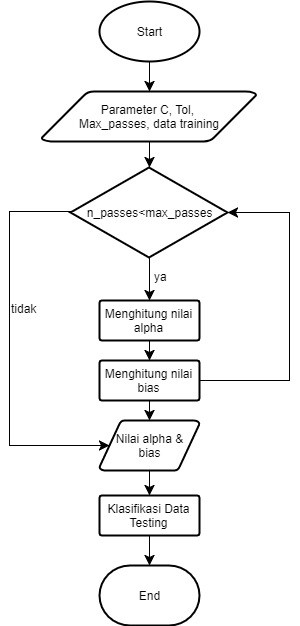
\includegraphics[width=10cm,height=13cm]{images/SVM.jpg}}	
	\captionof{figure}{\textit{Flowchart} Klasifikasi \textit{Support Vector Machine} (SVM) dengan SMO}
\end{minipage}
\end{adjustbox}

\noindent Berikut ini adalah contoh perhitungan klasifikasi teks pada Twitter kelas netral dengan data \textit{training} sebagai berikut:
\begin{table}[H]
	\caption{Data \textit{Training}}
	\centering
	\small
	\begin{adjustbox}{width=1\textwidth}
	\begin{tabular}{|p{2.5cm}|p{1.5cm}|p{1.5cm}|p{1.5cm}|p{1.5cm}|p{1.5cm}|p{1cm}|}
		\hline
		\multirow{2}{*}{\textbf{Dokumen}} & \multicolumn{5}{c|}{\textbf{Kata}}& \multirow{2}{*}{\textbf{Kelas}}\\
		\cline{2-6}
		& \textbf{DPR} & \textbf{Sukses} & \textbf{Semoga} & \textbf{Bagus} & \textbf{Jelek} & \\
		\hline
		D1 & 0.01 & 0.02 & 0.04 & 0.02 & 0.03 & 1 \\
		\hline
		D2 & 0 & 0.003 & 0.02 & 0.01 & 0 & 1 \\
		\hline
		D3 & 0.02 & 0.01 & 0 & 0.01 & 0 & -1 \\
		\hline
		D4 & 0.02 & 0 & 0.03 & 0.04 & 0.05 & -1 \\
		\hline
		D5 & 0 & 0.03 & 0.02 & 0.01 & 0.02 & 1 \\
		\hline
	\end{tabular}
	\end{adjustbox}
\end{table}

\noindent Berikut ini adalah data \textit{testing }yang akan digunakan untuk klasifikasi:

\begin{table}[H]
	\caption{Data \textit{Testing}}
	\centering
	\small
	\begin{adjustbox}{width=1\textwidth}
	\begin{tabular}{|p{2.5cm}|p{1.5cm}|p{1.5cm}|p{1.5cm}|p{1.5cm}|p{1.5cm}|p{1cm}|}
		\hline
		\multirow{2}{*}{\textbf{Dokumen}} & \multicolumn{5}{c|}{\textbf{Kata}}& \multirow{2}{*}{\textbf{Kelas}}\\
		\cline{2-6}
		& \textbf{DPR} & \textbf{Sukses} & \textbf{Semoga} & \textbf{Bagus} & \textbf{Jelek} & \\
		\hline
		T1 & 0.03 & 0 & 0.03 & 0.02 & 0 & ?\\
		\hline
	\end{tabular}
	\end{adjustbox}
\end{table}
Pada tabel 3.30, kelas 1 menunjukan kelas opini positif, sedangkan kelas -1 menunjukkan kelas opini lainnya. Proses dimulai dengan menghitung \textit{kernel} linear dengan menggunakan rumus tabel 2.7. Berikut ini contoh perhitungan nilai \textit{kernel} data \textit{training }pada tabel 3.30:
\begin{table}[H]
	\centering
	\small
	\begin{adjustbox}{width=1\textwidth}
	\begin{tabular}{|p{13.55cm}|}
		\hline
		K(D1,D2) = (0.01*0.01) + (0.02*0.02) + (0.04*0.04) + (0.02*0.02) + 
		(0.03*0.03) = 0.0034\\
		K(D1,D2) = (0.01*0) + (0.02*0.003) + (0.04*0.02) + (0.02*0.01) + (0.03*0) = 0.00106\\
		K(D1,D3) = (0.01*0.02) + (0.02*0.01) + (0.04*0) + (0.02*0.01) + (0.03*0) = 0.0006\\
		K(D1,D4) = (0.01*0.02) + (0.02*0) + (0.04*0.03) + (0.02*0.04) + (0.03*0.05) = 0.0037\\
		K(D1,D5) = (0.01*0) + (0.02*0.03) + (0.04*0.02) + (0.02*0.01) + (0.03*0) = 0.0022 
		\\
		\hline
	\end{tabular}
	\end{adjustbox}
\end{table}
\noindent Berikut ini adalah tabel hasil dari perhitungan \textit{kernel} pada setiap dokumen:
\begin{table}[H]
	\caption{Hasil Perhitungan \textit{Kernel} Linear pada Data \textit{Training}}
	\centering
	\small
	\begin{adjustbox}{width=1\textwidth}
	\begin{tabular}{|p{2cm}|p{2cm}|p{2cm}|p{1.9cm}|p{1.9cm}|p{1.5cm}|}
		\hline
		& \textbf{D1} & \textbf{D2} & \textbf{D3} & \textbf{D4} & \textbf{D5} \\
		\hline
		\textbf{D1} & 0.0034 & 0.00106 & 0.0006 & 0.0037 & 0.0022 \\
		\hline
		\textbf{D2} & 0.00106 & 0.000509 & 0,00013 & 0.001 & 0.00059 \\
		\hline
		\textbf{D3} & 0.0006 & 0.00013 & 0.0006 & 0,0008 & 0.0004 \\
		\hline
		\textbf{D4} & 0.0037 & 0.001 & 0.0008 & 0.0054 & 0.002 \\
		\hline
		\textbf{D5} & 0.0022 & 0.00059 & 0.0004 & 0.002 & 0.0018 \\
		\hline
	\end{tabular}
	\end{adjustbox}
\end{table}
Setelah mendapatkan perhitungan \textit{kernel} linear tahap selanjutnya mencari nilai alpha dan bias dengan algoritme \textit{Simplified} SMO sebagai berikut:
\begin{table}[H]
	\centering
	\small
	\begin{adjustbox}{width=1\textwidth}
	\begin{tabular}{|p{13.55cm}|}
		\hline
		\begin{enumerate}[label={},leftmargin=*,noitemsep]
			\item C=0.05 (Parameter Regularisasi)
			\item Tol=0.0001 (Toleransi Numerik)
			\item maxIter= 2 (maksimal pengulangan yang dilakukan ketika alpha tidak berubah)
			\item $\alpha_{i}$= 0
			\item $\alpha_{i}$(old)= 0
			\item b=0
			\item iter=0
			\item iter $<$ maxIter //kondisi while
			\begin{enumerate}[label={},noitemsep]
				\item jum\_perubahan\_alpha = 0
				\item i = 1//loop sebanyak jumlah dokumen \textit{training}
				\begin{enumerate}[label={},noitemsep]
					\item E$_{i}$ = f(x$_{1}$) - y$_{1}$
					\item = $[$((0 * 1 * 0.0034) + (0 * 1 * 0.000106) + (0 * -1 * 0.0006) + (0 * -1 * 0.0037) 
					+ (0 * 1 * 0.0022)) + 0$]$ - 1
					\item //kondisi if terpenuhi
					\item j = 3 //pilih j random, j != i
					\item E$_{3}$ = f(x$_{3}$) - y$_{3 }$
					\item = $[$((0 * 1 * 0.0006) + (0 * 1 * 0.00013) + (0 * -1 * 0.0006) + (0 * -1 * 0.0008) + (0 * 1 * 0.0004)) + 0$]$ - -1
					\item = 1
					\item $\alpha_{1}$(old) = 0
					\item $\alpha_{3}$(old) = 0
					\item L = max(0,(0-0))=0
					\item H = min(0.05,(0.0.5 + 0 - 0)) = 0.05
					\item //kondisi L!=H //kondisi L!=H terpenuhi
					\item $\eta$ = 2 * 0.06 - 0.16 - 0.09 = (-0.13)
					\item //kondisi eta $<$ 0 terpenuhi
					\item $\alpha_{3}$= 0 - $[$ ((-1 * (-1 - 1))) / (-0.13) $]$ = 15.385
					\item kondisi $\alpha_{3}>$ H terpenuhi
					\item $\alpha_{3}$= 0.05
					\item // kondisi abs($\alpha_{3}$ - $\alpha_{3}$(old)) $>$ 10$^{-5}$ terpenuhi
					\item $\alpha_{ 1 }$= 0 + (1 * -1 * (0 - 0.05)) = 0.05
					\item b$_{1 }$= 0 - (-1) - (1 * (0.05 - 0) * 0.16) - 
					(-1 * (0.05 - 0) * 0.06) = 0.995
					\item b$_{2}$ = 0 - (1) - (1 * (0.05 - 0) * 
					0.06) - (-1 * (0.05 - 0) * 0.09) = -0.9985
					\item b = (0.995 + (-0.9985))/2 = -0.0035
					\item jum\_perubahan\_alpha = 1
								
				\end{enumerate}
				\item //pengulangan dilakukan terus sampai data ke i=5
				\item iter = 0 // kondisi jum\_perubahan\_alpha !=0	
			\end{enumerate}
			\item //pengulangan dilakukan terus sampai kondisi while tidak terpenuhi 	
		\end{enumerate}
		\\
		\hline
	\end{tabular}
	\end{adjustbox}
\end{table}
\noindent Berikut ini adalah nilai alpha dan bias dari perhitungan \textit{simplified} SMO:

\begin{table}[H]
	\caption{Nilai Alpha dan Bias pada perhitungan SMO}
	\centering
	\small
	\begin{adjustbox}{width=1\textwidth}
	\begin{tabular}{|p{1.87cm}|p{1.87cm}|p{1.87cm}|p{1.87cm}|p{1.87cm}|p{2cm}|}
		\hline
		$\alpha_{1}$ & $\alpha_{2}$ & $\alpha_{3}$ & $\alpha_{4}$ & $\alpha_{5}$ & bias\\
		\hline
		0.78 & 0.5 & 0.3 & 0.21 & 0.25 & 0.135 \\
		\hline
	\end{tabular}
	\end{adjustbox}
\end{table}

Setelah mendapatkan nilai alpha dan bias, maka dapat dilakukan klasifikasi teks pada tabel 3.31. Perhitungan klasifikasi \textit{testing} juga dilakukan dengan perhitungan \textit{kernel} linear sebagai berikut:
\begin{table}[H]
	\centering
	\small
	\begin{adjustbox}{width=1\textwidth}	
	\begin{tabular}{|p{13.55cm}|}
		\hline
		K(T1,D1) = (0.03*0.01) + (0*0.02) + (0.03*0.04) + (0.02*0.02) + (0*0.03) = 0.0019\\
		K(T1,D2) = (0.03*0) + (0*0.03) + (0.03*0.02) + (0.02*0.01) + 
		(0*0) = 0.0008\\
		K(T1,D3) = (0.03*0.02) + (0*0.01) + (0.03*0) + (0.02*0.01) 
		+ (0*0) = 0.0008\\
		K(T1,D4) = (0.03*0.02) + (0*0) + (0.03*0.03) + 
		(0.02*0.04) + (0*0.05) = 0.0023\\
		K(T1,D5) = (0.03*0) + (0*0.03) + (0.03*0) 
		+ (0.02*0.03) + (0*0.02) = 0.0008 \\
		\hline
	\end{tabular}
	\end{adjustbox}
\end{table}
\noindent Berikut ini adalah hasil perhitungan \textit{kernel }linear pada data \textit{testing} : 

\begin{table}[H]
	\caption{Hasil Perhitungan \textit{Kernel} Linear pada Data \textit{Testing}}
	\centering
	\small
	\begin{adjustbox}{width=1\textwidth}
	\begin{tabular}{|p{2cm}|p{2cm}|p{2cm}|p{1.9cm}|p{1.9cm}|p{1.5cm}|}
		\hline
		& \textbf{D1} & \textbf{D2} & \textbf{D3} & \textbf{D4} & \textbf{D5} \\
		\hline
		\textbf{T1} & 0.0019 & 0.0008 & 0.0008 & 0.0023 & 0.0008 \\
		\hline
	\end{tabular}
	\end{adjustbox}
\end{table}
\noindent Setelah perhitungan \textit{kernel} linear dilakukan maka dapat dilakukan perhitungan klasifikasi sebagai berikut:
\begin{table}[H]
	\centering
	\small
	\begin{adjustbox}{width=1\textwidth}	
	\begin{tabular}{|p{13.55cm}|}
		\hline
		F(x) = (0.78 * 1 * 0.0019) + (0.5 * 1 * 0.0008) + (0.3 * -1 * 0.0008) + (0.21 * -1 * 0.0023) + (0.25 * 1 * 0.0008) + 0.135 = -1.86 = -1 \\
		\hline
	\end{tabular}
	\end{adjustbox}
\end{table}
Berdasarkan perhitungan di atas, dokumen T1 termasuk dalam kelas 1 yang merupakan kelas bukan netral.
\pagebreak
\subsection{\textit{Class Diagram}}
Berikut ini adalah \textit{design} \textit{class diagram} pada sistem analisis sentimen yang akan dibuat:

	
\begin{adjustbox}{width=1\textwidth}
\noindent\begin{minipage}{\linewidth}
	\framebox[\textwidth]{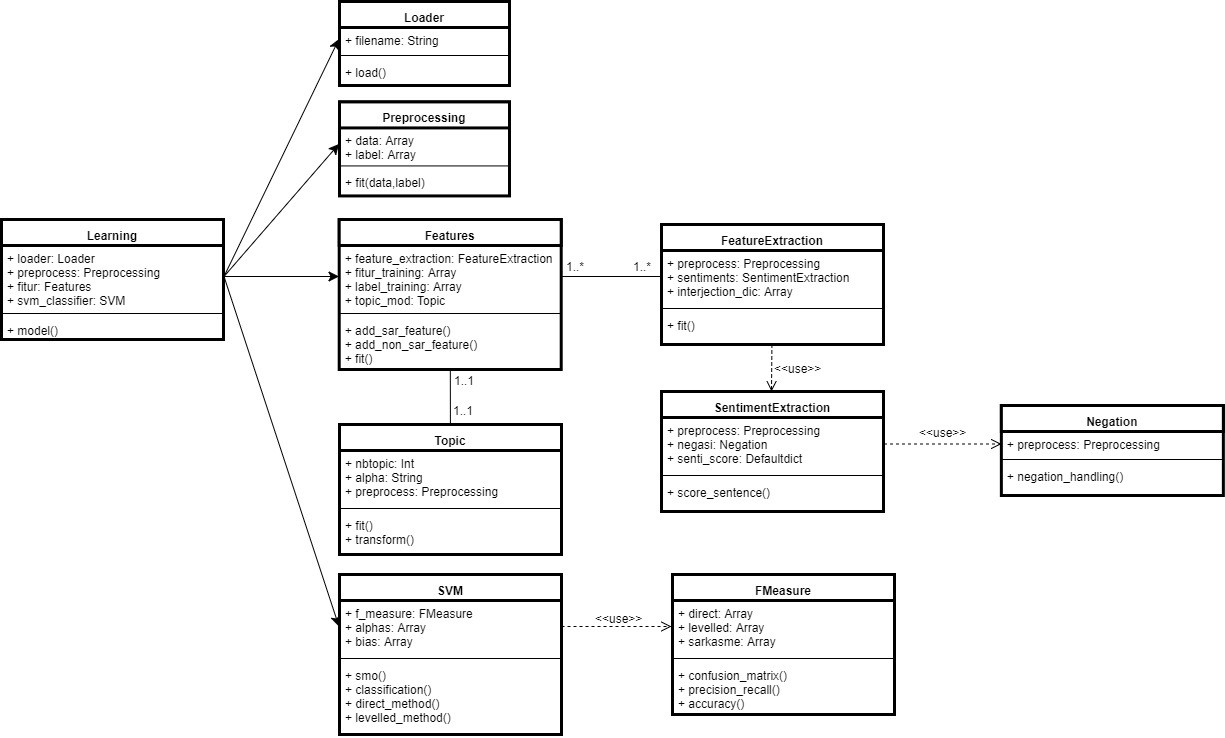
\includegraphics[width=13cm]{images/class_diagram.jpg}}	
	\captionof{figure}{\textit{Class Diagram} Sistem Analisis Sentimen}
\end{minipage}
\end{adjustbox}
\newpage